\documentclass{standalone}

\usepackage{tikz}
\usepackage{circuitikz}

\tikzset{block/.style = {draw, fill=white, very thick, rectangle, minimum height=1cm, minimum width=2cm},
         lblock/.style={draw,fill=white,very thick, rectangle, minimum height=3cm, minimum width=1cm},
         sum/.style= {draw, fill=white, very thick, circle, node distance=0.5cm}}

         
\begin{document}
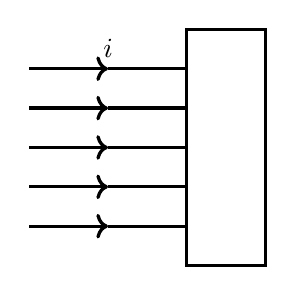
\begin{tikzpicture}[scale=2]
    \node[lblock](c)at(-0.25,0){};
    \draw[->,very thick](-1.5,0)--(-1,0);
    \draw[-,very thick](-1,0)--(-0.5,0);
    \draw[->,very thick](-1.5,0.25)--(-1,0.25);
    \draw[-,very thick](-1,0.25)--(-0.5,0.25);
    \draw[->,very thick](-1.5,0.5)--(-1,0.5);
    \draw[-,very thick](-1,0.5)node[above]{$i$}--(-0.5,0.5);
    \draw[->,very thick](-1.5,-0.25)--(-1,-0.25);
    \draw[-,very thick](-1,-0.25)--(-0.5,-0.25);
    \draw[->,very thick](-1.5,-0.5)--(-1,-0.5);
    \draw[-,very thick](-1,-0.5)--(-0.5,-0.5);
\end{tikzpicture}
\end{document}